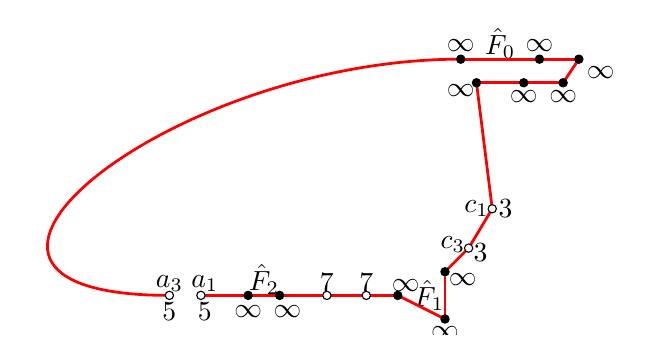
\begin{tikzpicture}[line cap=round,line join=round,x=1cm,y=1cm]
\clip(-3,1.5) rectangle (4.5,5.4);

\begin{scriptsize}




%
% Node F_0
%
\draw (3,5.2) node {\normalsize $\hat F_0$};
\draw [line width=1pt,color=red] (2.7,4.7) to  (3.8,4.7); 
\draw [line width=1pt,color=red] (3.8,4.7) to  (4,5); 
\draw [line width=1pt,color=red] (4,5) to  (2.5,5); 

\draw [line width=1pt,color=red] (2.5,5) to[in=180,out=180,looseness=2]  (-1.2,2); 

%^c
\draw [line width=1pt,color=red] (2.6,2.6) to  (2.9,3.1);
\draw [line width=1pt,color=red] (2.7,4.7) to  (2.9,3.1);

\draw (-1.2,2.15) node {\normalsize $a_3$};
\draw (-1.2,1.8) node {\normalsize $5$};
\draw [fill=white] (-1.2,2)circle (1.5pt);
\draw (2.7,3.1) node {\normalsize $c_1$};
\draw (3.07,3.1) node {\normalsize $3$};
\draw [fill=white] (2.9,3.1)circle (1.5pt);



\draw (2.5,5)[anchor=south] node {\normalsize $\infty$};
\draw [fill=black] (2.5,5)circle (1.5pt);
\draw (2.5,4.6) node {\normalsize $\infty$};
\draw [fill=black] (2.7,4.7)circle (1.5pt);
\draw (3.5,5)[anchor=south] node {\normalsize $\infty$};
\draw [fill=black] (3.5,5)circle (1.5pt);
\draw (4,5)[anchor=north west] node {\normalsize $\infty$};
\draw [fill=black] (4,5)circle (1.5pt);
\draw (3.8,4.7)[anchor=north] node {\normalsize $\infty$};
\draw [fill=black] (3.8,4.7)circle (1.5pt);
\draw (3.3,4.7)[anchor=north] node {\normalsize $\infty$};
\draw [fill=black] (3.3,4.7)circle (1.5pt);




%
% Node F_1
%
\draw (2.1,2) node {\normalsize $\hat F_1$};
%node path
\draw [line width=1pt,color=red] (2.3,2.3) to  (2.3,1.7); 
\draw [line width=1pt,color=red] (1.7,2) to  (2.3,1.7); 

\draw [line width=1pt,color=red] (2.6,2.6) to  (2.3,2.3); 
\draw [line width=1pt,color=red] (1.7,2) to  (1.3,2); 

% F_1 to F_2
\draw [line width=1pt,color=red] (.8,2) to  (1.3,2); 

\draw (1.8,2.13) node {\normalsize $\infty$};
\draw [fill=black] (1.7,2)circle (1.5pt);
\draw (2.3,1.7)[anchor=north] node {\normalsize $\infty$};
\draw [fill=black] (2.3,1.7)circle (1.5pt);
\draw (2.25,2.2)[anchor=west] node {\normalsize $\infty$};
\draw [fill=black] (2.3,2.3)circle (1.5pt);
\draw (1.3,2.16) node {\normalsize $7$}; %b_3
\draw [fill=white] (1.3,2)circle (1.5pt);

\draw (2.4,2.65) node {\normalsize $c_3$};
\draw (2.75,2.55) node {\normalsize $3$};
\draw [fill=white] (2.6,2.6)circle (1.5pt);

%
% Node F_2
%
\draw (0,2.2) node {\normalsize $\hat F_2$};

\draw [line width=1pt,color=red] (-.8,2) to  (-.3,2); 
\draw [line width=1pt,color=red] (.8,2) to  (.3,2);   
\draw [line width=1pt,color=red] (-.3,2) to (.3,2);   

\draw [fill=black] (-.2,2) circle (1.5pt);
\draw (-.2,1.8) node {\normalsize $\infty$};
\draw [fill=black] (.2,2) circle (1.5pt);
\draw (.3,1.8) node {\normalsize $\infty$};
\draw (-.75,2.15) node {\normalsize $a_1$};
\draw [fill=white] (-.8,2) circle (1.5pt);
\draw (-.75,1.8) node {\normalsize $5$};
\draw (.8,2.16) node {\normalsize $7$}; %b_1
\draw [fill=white] (.8,2) circle (1.5pt);

\end{scriptsize}
\end{tikzpicture}
